\documentclass[11pt,a4paper]{article}
\usepackage[T1]{fontenc}
\usepackage{graphicx}
\usepackage{mathtools}
\usepackage{amssymb}
\usepackage{geometry}
\usepackage{titlesec}
\usepackage{enumitem} % 添加enumitem宏包
\usepackage{amsfonts}
\usepackage{amssymb}
\usepackage{fancyhdr} % 添加fancyhdr宏包
\usepackage{lastpage} % 添加lastpage宏包
\usepackage{graphicx} % 导入graphicx包
\usepackage{gensymb} % 引入gensymb包
\usepackage[UTF8]{ctex}
% 应用fancyhdr宏包的页脚样式
\pagestyle{fancy}
\fancyhf{} % 清除当前的页眉页脚设置
\fancyfoot[L]{免费开源,请勿商用} % 页脚左下方显示文字
\fancyfoot[R]{作者:阿尧} % 页脚右下方显示文字
\renewcommand{\headrulewidth}{0pt} % 去掉页眉的横线
\renewcommand{\footrulewidth}{1pt} % 设置页脚的横线宽度
\usepackage{draftwatermark} %增加水印
\SetWatermarkText{本真题由b站up陈瀚尧探索世界免费开源}
\SetWatermarkScale{0.3} % 可以调整为合适的大小
\SetWatermarkColor{gray!50} % 灰色透明度为50%

% 设置更窄的页面边距
\geometry{left=3cm, right=3cm, top=1cm, bottom=2cm}

% 设置section标题格式
\titleformat{\title}{\bfseries}{\thetitle}{1em}{}

% 设置section之间的距离
\titlespacing*{\section}{0pt}{3.25ex plus 1ex minus .2ex}{1.5ex plus .2ex}

\begin{document}
    \title{中国科学院大学\\2018年招收攻读硕士学位研究生入学统一考试试题\\科目名称:光学}
    \author{制作者:b站up 陈瀚尧探索世界}
    \date{}
    \maketitle
    % 设置section标题不显示序号
    \titleformat{\section}[block]{\normalfont\Large\bfseries}{}{0pt}{}

    % 设置itemize环境的项目符号为空
    \setlist[itemize]{label=} 

    \section{考试须知:}
    \begin{itemize}[topsep=0pt,itemsep=0pt,partopsep=0pt]
        \item 1.本试卷满分为150分,全部考试时间总计180分钟。
        \vspace{-3mm}
        \item 2.所有答案必须写在答题纸上,写在试题纸上或草稿纸上一律无效。
        \vspace{-3mm}
        \item 3.可以使用无字典存储或编程功能的电子计算器。(此条对于25考研可能作废)
    \end{itemize}
    \vspace{-5mm}
    \noindent\rule{\textwidth}{0.5pt} % 添加一条线
    \vspace{-12mm}
    \section*{一、简答题}
    \begin{enumerate}
        \vspace{0mm}
        \item 简述光的直线传播定律、光的独立传播定律、反射定律和折射定律。
        \vspace{5mm}
        \item 光学系统的焦点、焦平面、主点、主平面、节点的定义。
        \vspace{5mm}
        \item 什么是孔径光阑、视场光阑、渐晕光阑和消杂光光阑?
        \vspace{5mm}
        \item 伽利略望远镜和开普勒望远镜的主要区别是什么?
        \vspace{5mm}
    \end{enumerate}
    \subsection*{2.如图所示,由折射率均为1.5的棱镜和凸薄透镜组成理想光学系统。高度为$1mm$的物体置于距棱镜平面的垂直距离$QB=6cm$的光轴上Q点,棱镜的$\angle BAC=45\degree$,$BC=3cm$,$CD=4cm$。棱镜曲面的半径为$5cm$,棱镜球面定点D与凸薄透镜光心O的距离为$DO=40cm$,凸薄透镜两个球面的半径均为$30cm$,在旁轴条件下该系统最后成像的位置和高度,以及像的倒正和虚实。}
    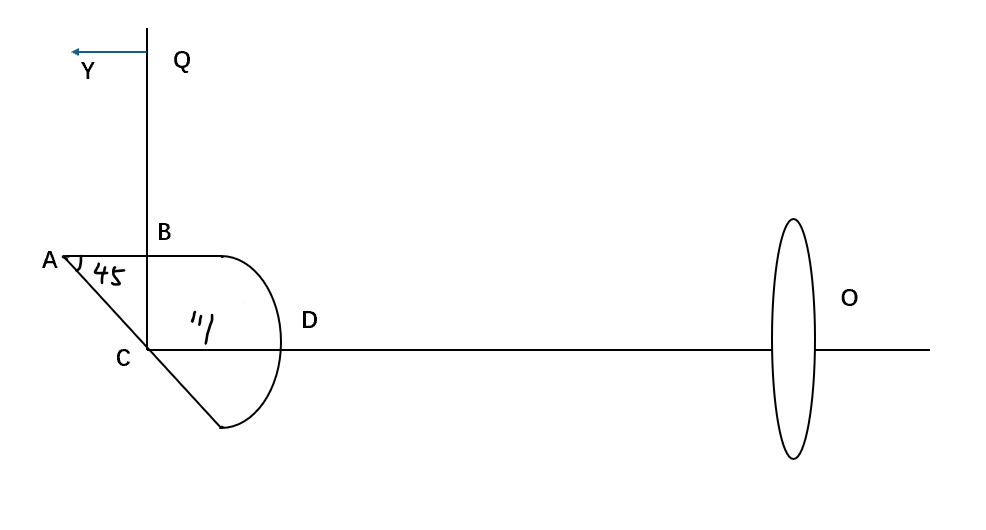
\includegraphics[scale=0.2]{1.png}% 插入图片,按50%的比例缩放
    \vspace{10mm}
    \subsection*{3.两个薄透镜L1和L2,口径分别为6cm和4cm,焦距分别为$f_{1}^{'}=9cm$,$f_{2}^{'}=5cm$,相距5cm。在L1和L2之间,距离L2为2cm处放入一个带有直径为6cm小孔的光阑AB,物点位于L1前方12cm处。求孔径光阑、入瞳和出瞳。}
    \vspace{10mm}
    \subsection*{4.有一焦距为50cm,口径为50mm的放大镜,眼睛到它的距离为125mm,如果物体经放大镜后所成的像在明视距离处,求此时放大镜的视放大率。}
    \vspace{10mm}
    \subsection*{5.试写出长短轴之比为2:1、长轴沿x轴的右旋和左旋椭圆偏振光的归一化琼斯矢量,并计算该二偏振光合成光的偏振状态。(偏振光的旋向按逆光传播方向观察规定)}
    \vspace{10mm}
    \subsection*{6.一束右旋圆偏振光的光强为$I_{0}$,由空气垂直入射到玻璃上,空气和玻璃的折射率分别为$n_1=1$和$n_2=1.5$,试由入射光导出反射光的光场表达式、偏振态和光强。}
    \vspace{10mm}
    \subsection*{7.在杨氏双缝干涉实验中,照明光波长$\lambda =500nm$,双缝$S_1$和$S_2$相距$d=0.5mm$,观察屏距双缝$r_0=1m$。}
    \begin{itemize}
        \vspace{0mm}
        \item (1)当如图所示,以厚度$t=0.02mm$、折射率$n=1.56$的透明薄片贴住小孔$S_1$时,确定屏上干涉条纹相对不贴薄片时的变化;
        \vspace{0mm}
        \item (2)当照明光变为波长宽度$\vartriangle \lambda=0.05nm$的准单色光时,薄片为多厚可使观察屏上$P_0$点附件的干涉条纹消失。
        
        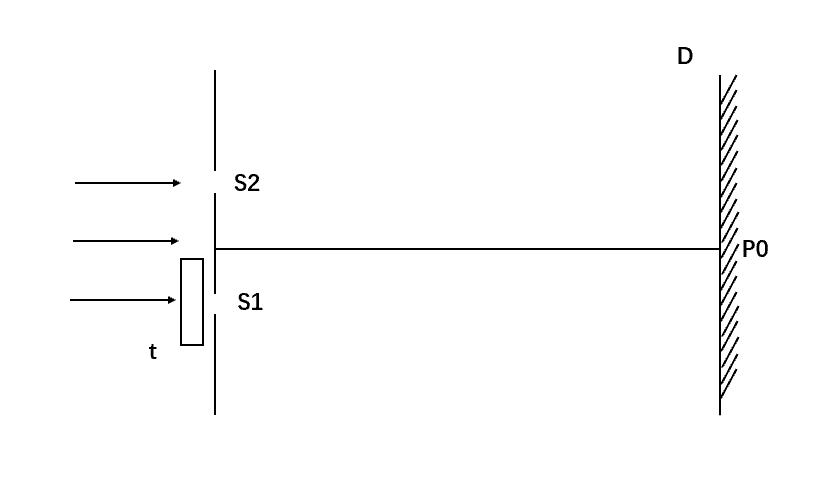
\includegraphics[scale=0.2]{2.png}% 插入图片,按50%的比例缩放
    \end{itemize}
    \vspace{20mm}
    \subsection*{8.今有一干涉滤波片,其间隔层厚度为$2x10^{-4}mm$,折射率$n=1.5$,高反膜的反射率$R=0.9$。试求:}
    \begin{itemize}
        \vspace{0mm}
        \item (1)光波正入射时,滤波片在可见光区的中心波长及其透射带的波长半宽度;
        \vspace{0mm}
        \item (2)当光波以$10\degree$角斜入射时,滤光片在可见光的透射光波长。
        \vspace{0mm}
    \end{itemize}
    \vspace{20mm}
    \subsection*{9.今有一束直径为2mm的红宝石激光($\lambda=694.3nm$)自地面射向月球,已知地面-月球距离为$3.76x10^{5}km$,试问在月球上的光斑有多大?如果反向运用望远镜将激光束扩束成$2m$直径,则望远镜的倍数为多少?此时照射到月球上的光斑为多大?}
    \vspace{10mm}
    \subsection*{10.试求一宽为$5cm$,每毫米内有400条刻线的光栅,对于波长为$500nm$入射光的一级角色散率。今若入射光与栅平面法线成$30\degree$角方向斜入射,求该光栅能分辨的谱线的最小波长差是多少?}
    \vspace{10mm}
    \subsection*{11.如图所示,两块晶体(主折射率$n_0=1.5246$,$n_e=1.4796$,厚度$d=2cm$)平行薄板按相同方式切割(图中斜线代表光轴方向,与通光面法线成$45\degree$角),并平行放置。今有一波长为$\lambda=500nm$的细平面自然光垂直入射晶体,试计算并绘图说明晶体中o光和e光的传播光路,偏振态及在第二个晶体出射面上两个光的相位差。}
    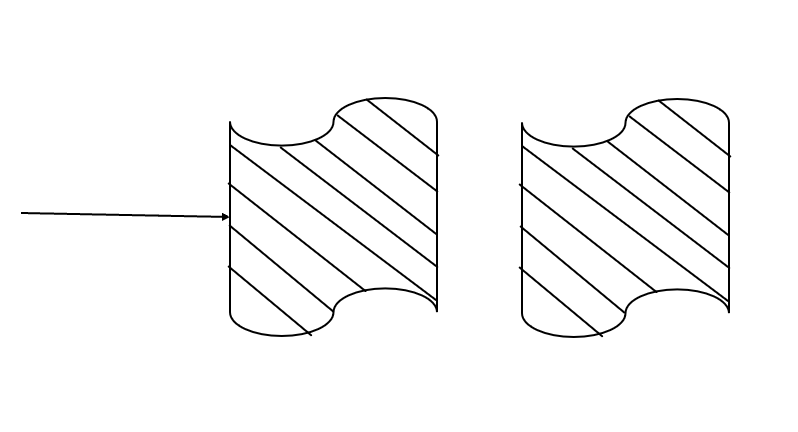
\includegraphics[scale=0.2]{3.png}% 插入图片,按50%的比例缩放
    \vspace{10mm}
    \subsection*{12.一束波长为$\lambda_{2}=706.5nm$的左旋圆偏振光入射到相应于$\lambda_1=404.6nm$的方解石$\frac{1}{4}$波片上,试求出射光束的偏振态。已知方解石对$\lambda_1$光的$n_o=1.6813$,$n_e=1.4969$;对$\lambda_2$光的$n_o=1.6521$,$n_e=1.4836$。}
    \vspace{10mm}
\end{document}